\documentclass[conference]{IEEEtran}
% \IEEEoverridecommandlockouts
% The preceding line is only needed to identify funding in the first footnote. 
% If that is unneeded, please comment it out.

\usepackage{cite}
\usepackage{amsmath,amssymb,amsfonts}
\usepackage{algorithmic}
\usepackage{graphicx}
\usepackage{textcomp}
\usepackage{xcolor}
\usepackage{url}
\usepackage{listings}
\usepackage{algorithm2e}
\usepackage{hyperref}

\hypersetup{
    colorlinks=true,
    urlcolor=blue,
}

% Configure the listings package
\lstset{
    basicstyle=\ttfamily\scriptsize,
    keywordstyle=\color{orange},
    commentstyle=\color{gray},
    stringstyle=\color{red},
    numbers=left,
    numberstyle=\tiny\color{gray},
    stepnumber=1,
    numbersep=5pt,
    showspaces=false,
    showstringspaces=false,
    breaklines=true,
    frame=single,
    tabsize=2,
    captionpos=b,
    columns=flexible,
    keepspaces=true
}

\def\BibTeX{{\rm B\kern-.05em{\sc i\kern-.025em b}\kern-.08em
    T\kern-.1667em\lower.7ex\hbox{E}\kern-.125emX}}

\begin{document}

\title{Kingdomino: Enter the Virtual World}

\author{\IEEEauthorblockN{Hai Duong, Tran}
    \IEEEauthorblockA{\textit{CSE, Frankfurt University of Applied Sciences} \\
        Frankfurt am Main, Germany \\
        hai.tran2@stud.fra-uas.de}
    \and
    \IEEEauthorblockN{Pham Minh Tuan, Bui}
    \IEEEauthorblockA{\textit{CSE, Frankfurt University of Applied Sciences} \\
        Frankfurt am Main, Germany \\
        pham.bui@stud.fra-uas.de}
}

\maketitle

\begin{abstract}
    This paper presents a digital adaptation of the board game Kingdomino,
    developed using Java and the LibGDX framework. Our implementation leverages an
    event-driven architecture, a flood-fill algorithm for scoring, and shader-based
    rendering to enhance the user experience. We explore key aspects of game logic,
    including tile placement validation, turn-based mechanics, and dynamic UI
    interactions. The paper details the design choices, algorithms, and modular
    structure of the system, ensuring efficiency and scalability. Additionally, we
    evaluate game performance through experimental results and discuss future
    improvements, such as AI integration and multiplayer capabilities.
\end{abstract}

\begin{IEEEkeywords}
    Kingdomino, boardgame, implementation, game development, OOP
\end{IEEEkeywords}

%======================================================
\section{Introduction}
% 1. INTRODUCTION
% -- Explain overall motivation, background, and significance.
% -- Provide a quick overview of the Kingdomino game and the goals of your project.

Kingdomino~\cite{wiki:kingdomino} is a strategic tile placement game where
players act as lords expanding their kingdoms. The objective is to construct
the most prosperous territory by selecting and placing tiles that represent
various terrain types, such as wheat fields, lakes, and mountains. Each tile
comprises two sections that must be connected to the existing kingdom based on
matching terrain types.

This paper presents a digital adaptation of Kingdomino, developed using Java
and the LibGDX framework. Our implementation leverages an event-driven
architecture, a flood-fill algorithm for scoring, and shader-based rendering to
enhance the user experience. We explore key aspects of game logic, including
tile placement validation, turn-based mechanics, and dynamic UI interactions.
The paper details the design choices, algorithms, and modular structure of the
system, ensuring efficiency and scalability. Additionally, we evaluate game
performance through experimental results and discuss future improvements, such
as AI integration and multiplayer capabilities.\footnote{The source code for
    the Kingdomino digital adaptation can be found on GitHub at
    \url{https://github.com/fuisl/kingdomino}.}

The paper is structured as follows: Section~\ref{sec:problem_description}
describes the problem and game mechanics. Section~\ref{sec:related_work}
reviews related work and algorithms. Section~\ref{sec:teamwork} discusses
teamwork and collaboration tools. Section~\ref{sec:proposed_approaches}
outlines the proposed approaches, including the event-driven architecture and
input handling. Section~\ref{sec:implementation_details} and
Section~\ref{sec:graphical_enhancement} detail the implementation, including
game states, tile placement, scoring mechanisms, graphical enhancements, and
visual effects. Section~\ref{sec:experimental_results} presents experimental
results and performance analysis. Finally, Section~\ref{sec:conclusions}
concludes the paper and suggests future work.

%======================================================
\section{Problem Description}
\label{sec:problem_description}
% 2. PROBLEM DESCRIPTION
% -- Formal description: definitions, examples.
% -- Description of Kingdomino with examples.

The primary goal in Kingdomino is to construct the most prestigious kingdom by
strategically placing tiles within a constrained 5$\times$5 grid. Players must
explore various terrain types—fields, lakes, mountains, forests, meadows, and
swamps—and connect them to their existing kingdom while adhering to specific
placement rules. Each tile consists of two sections, and at least one section
must match the terrain type of an adjacent tile. Crowns on tiles act as
multipliers to the score of connected terrain groups, encouraging players to
prioritize valuable combinations.

Players compete for tiles through a selection mechanism that balances
high-value tiles with the consequence of selecting later in subsequent rounds.
This creates an optimization problem where players must maximize immediate
gains while strategically positioning themselves for future moves. The game
concludes when each player has filled their grid or can no longer place tiles,
with scoring determining the winner based on terrain connectivity and crown
placements.

\begin{figure}[htbp]
    \centerline{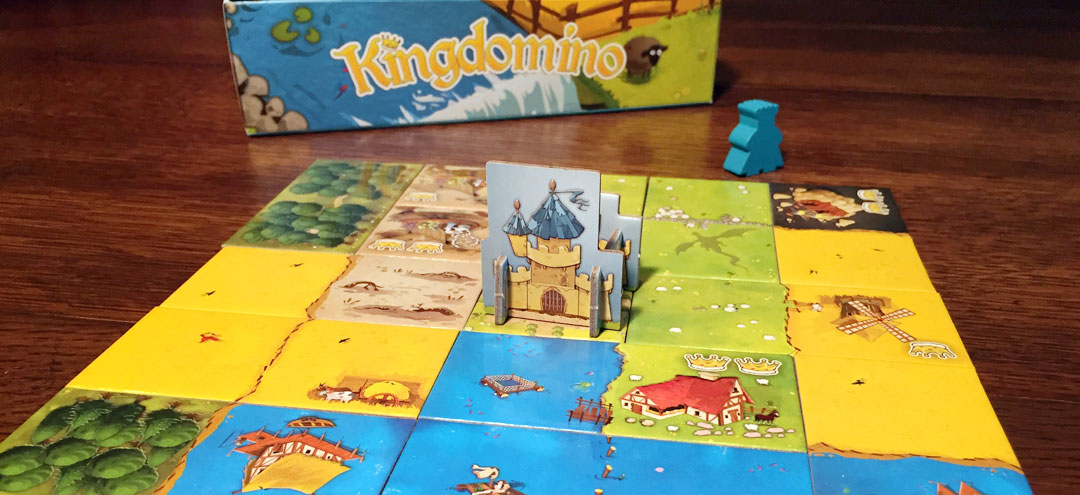
\includegraphics[width=0.5\textwidth]{assets/kingdomino.jpg}}
    \caption{Kingdomino Board Game.}\label{fig:kingdomino}
\end{figure}

\subsection{Formal Description}

The game involves the following components and constraints:

\subsubsection{Components}

\begin{itemize}
    \item \textbf{Tiles}: Each tile consists of two sections, each representing one of the six terrain types (fields, lakes, mountains, forests, meadows, and swamps). Certain tiles include crowns, which serve as score multipliers.
    \item \textbf{Kingdom}: A 5$\times$5 grid where tiles are placed. Each player starts with a central tile (wild type) and builds outward.
    \item \textbf{Selection Order}: Players select tiles in descending order of tile value (higher numbers first) and use their selection to determine the order in subsequent rounds.
\end{itemize}

\subsubsection{Rules}

\begin{itemize}
    \item \textbf{Placement}:
          \begin{itemize}
              \item Tiles must connect to at least one adjacent tile with the same terrain type
                    (horizontally or vertically).
              \item The grid is limited to 5$\times$5 dimensions; any tile that cannot be placed is
                    discarded.
          \end{itemize}

    \item \textbf{Scoring}:
          \begin{itemize}
              \item Points are calculated as the product of the number of connected tiles of the
                    same terrain and the number of crowns within the connected group.
              \item Bonuses include:
                    \begin{itemize}
                        \item +10 points for placing the central castle at the grid's center.
                        \item +5 points for completing a full grid.
                    \end{itemize}
          \end{itemize}

    \item \textbf{Game Variants}:
          \begin{itemize}
              \item A 7$\times$7 grid variant for advanced play.
              \item Multi-round gameplay (Dynasty mode) with cumulative scores.
          \end{itemize}
\end{itemize}

\subsubsection{Objective}

Maximize the total score by constructing a kingdom that balances large
connected terrain groups with crown placements, while competing against other
players for optimal tile selection.

\subsection{Examples of Gameplay}
% -- Provide short examples or scenarios that clarify the rules.

Gameplay is explain in Appendix~\ref{app:gameplay}.

%======================================================
\section{Related Work}
\label{sec:related_work}
% 3. RELATED WORK
% -- Discuss any algorithms or approaches that are relevant, 
%    e.g., fractals, data generation, evolutionary algorithms, etc.
% -- Mention similar or existing board games / AI approaches.
Board games like Carcassonne\cite{wiki:carcassonne} and
Patchwork\cite{wiki:patchwork} offer valuable insights into the mechanics of
tile placement and scoring, making them relevant to our implementation of
Kingdomino. Carcassonne challenges players to build cities, roads, and fields
by placing tiles based on terrain type, a mechanic that closely aligns with
Kingdomino’s terrain-matching rules. Similarly, Patchwork emphasizes the
efficient use of a constrained grid, much like Kingdomino’s 5×5 board, where
players must optimize placement for maximum scoring. These games demonstrate
how simple mechanics can result in complex decision-making, a feature we aim to
replicate in our project.

In addition to inspiration from traditional board games, the implementation of
Kingdomino leverages several key computational and architectural techniques.
The scoring mechanism, for instance, utilizes a flood-fill
algorithm\cite{wiki:floodfill} to evaluate the connected terrain groups and
their associated scores. This algorithm, commonly employed in image processing
and graph traversal\cite{wiki:graphtraversal}, provides an efficient way to
traverse and calculate properties of contiguous regions. Its application in
Kingdomino ensures accurate and performant scoring calculations, even as the
board becomes increasingly complex during gameplay.

The game is designed using an event-driven architecture\cite{wiki:eventdriven,
    wiki:floodfill}, where interactions, where interactions such as tile placement
and scoring updates are managed asynchronously through an EventManager. This
approach is prevalent in modern game frameworks and engines, such as LibGDX,
Unity, and Unreal Engine, and ensures a clear separation between game logic and
user input. By decoupling these components, the design achieves improved
modularity and scalability, enabling future enhancements such as AI integration
or multiplayer features. The intention was to implement Entity-Component-System
(ECS) architecture\cite{wiki:ecs} to further improve the game's performance and
scalability. But we not strictly follow this architecture for flexibility and
simplicity.

Furthermore, the aesthetic design of Kingdomino draws from pixel-art-inspired
games, including Balatro\cite{wiki:balatro}, which use vibrant colors and
minimalistic textures to create a visually engaging experience. This style has
been adopted to maintain the simplicity of the board game while enhancing the
digital adaptation with a modern and nostalgic visual appeal.

Finally, the use of the LibGDX framework\cite{libgdx} streamlines development,
particularly in rendering, asset management, and input handling. By leveraging
tools such as TextureAtlas\cite{wiki:textureatlas} for managing game assets and
InputMultiplexer for handling player interactions, the framework supports an
efficient implementation of Kingdomino's mechanics and aesthetics. This
integration aligns with industry-standard practices for creating scalable,
interactive applications.

Incorporating these approaches and inspirations, the implementation of
Kingdomino aims to balance simplicity, efficiency, and engagement, ensuring a
faithful and enjoyable digital representation of the original board game.

% Example referencing
% As noted by some authors \cite{exampleRef1}, 
% board games have often been used to benchmark AI approaches.

%======================================================
\section{Teamwork}
\label{sec:teamwork}
% -- Who did what, how the tasks were divided, how you communicated and tracked progress, 
%    brainstorming sessions, etc.

We divided the project into backend (game logic) and frontend (GUI), using
GitHub ecosystem for tracking and communication. We also followed SCRUM
planning techniques.\footnote{see our initial planning on GitHub Project at
    \url{https://github.com/users/fuisl/projects/15}}

% (Fig~\ref{fig:kanban}).
\begin{figure}[htbp]
    \centerline{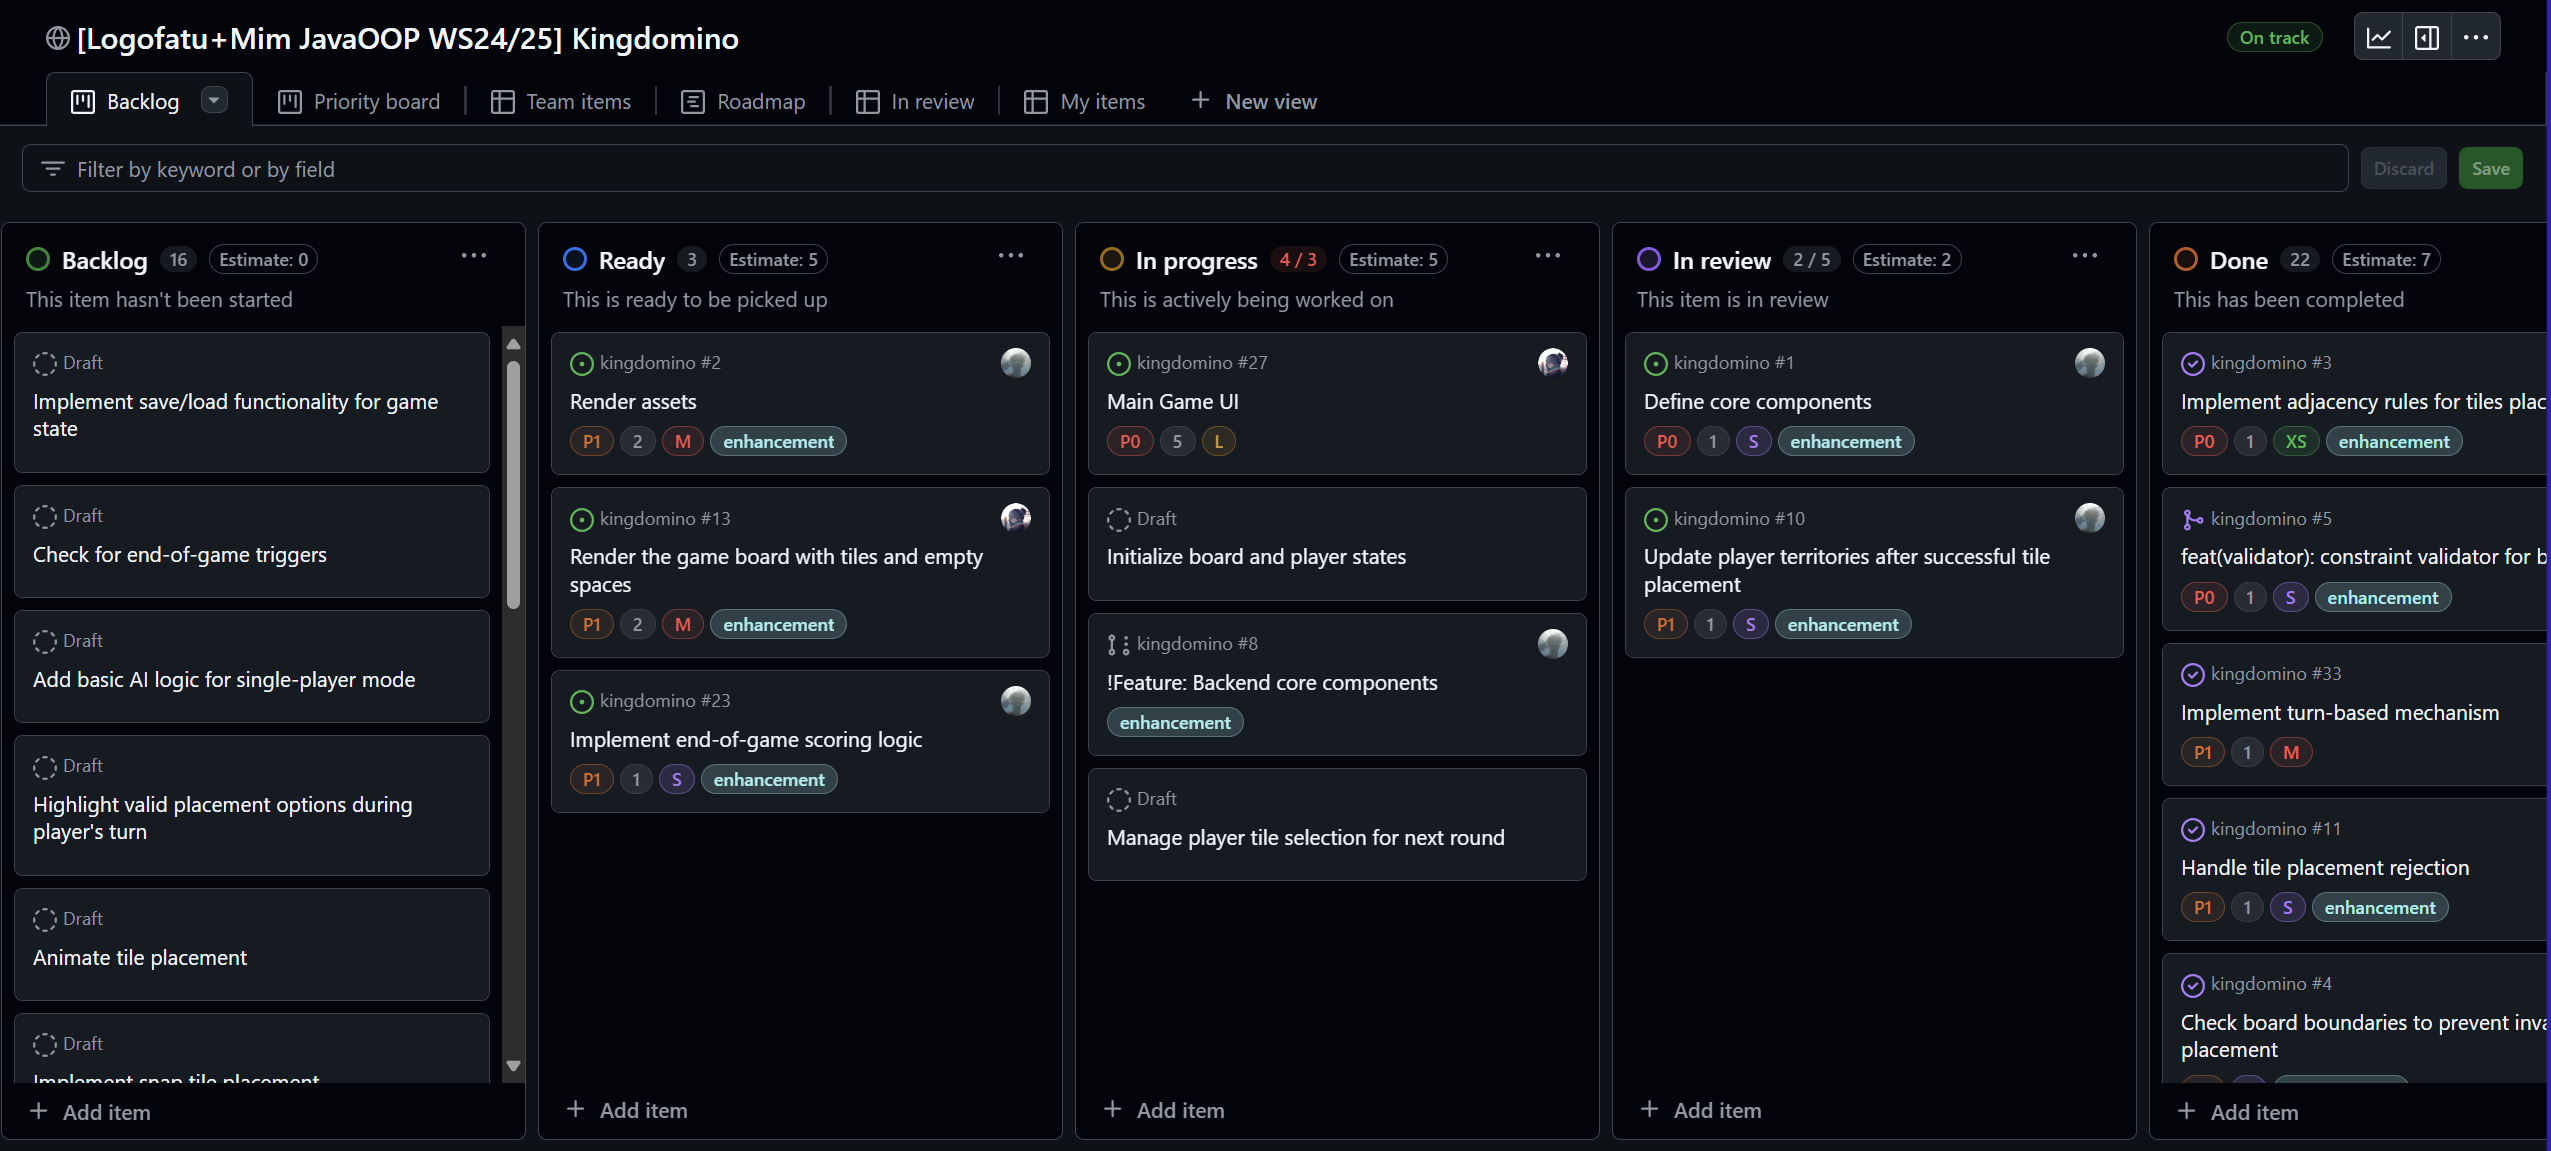
\includegraphics[width=0.5\textwidth]{assets/github-project.png}}
    \caption{Kanban Board implements SCRUM planning technique.}\label{fig:kanban}
\end{figure}

\subsection{Roles and Responsibilities}
Hai Duong Tran handled backend logic, including tile placement rules, scoring,
and game flow. He also integrated the flood-fill algorithm and worked on
shaders and effects. Pham Minh Tuan Bui focused on the GUI, rendering game
elements with LibGDX, and work on creating our original assets for this
project. He also worked on visual aesthetics. Both members contributed to the
success of this project.

We collaborated on various aspects not just within our scope and
responsibilities. We held regular meetings, and conducted code reviews to
maintain quality and consistency. This approach enhanced productivity and
understanding of the project.

\subsection{Collaboration Tools and Workflow}
Most of our communication happened on Github Issues and Pull Requests. The
tools are used for tracking and code reviews. Each member created branches for
their tasks, ensuring main branch stability. Code reviews were conducted via
GitHub Pull Requests (Fig~\ref{fig:github-pr}), maintaining code quality and
facilitating knowledge sharing. For communication, we used Messenger and
in-person meetings, documenting progress via commit messages and digital
drafts.

\subsection{Gitflow Workflow}
We adopted the Gitflow workflow for version control, which is an
industry-standard branching model for Git. This approach helps manage the
development process by organizing branches and ensuring a clear path from
development to production.

\begin{figure}[htbp]
    \centerline{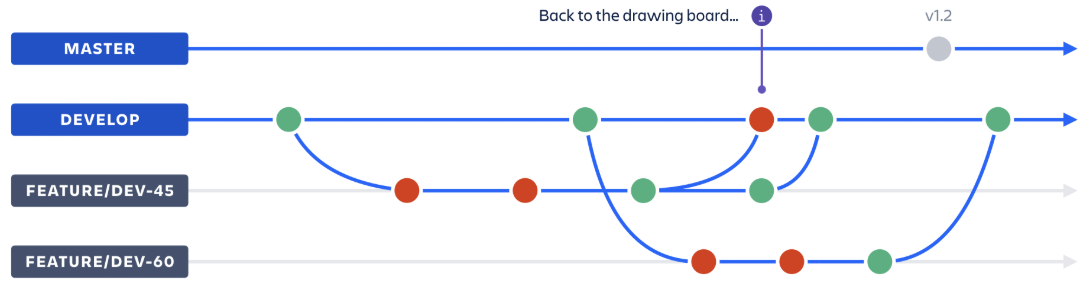
\includegraphics[width=0.48\textwidth]{assets/gitflow.png}}
    \caption{Gitflow Workflow.}\label{fig:gitflow}
\end{figure}

The Gitflow workflow consists of the following branches:
\begin{itemize}
    \item \textbf{main}: The main branch containing production-ready code.
    \item \textbf{dev}: The integration branch for features and fixes.
    \item \textbf{feature/*}: Branches for developing new features.
    \item \textbf{release/*}: Branches for preparing releases.
    \item \textbf{hotfix/*}: Branches for quick fixes to production code.
\end{itemize}

This workflow allows for parallel development, efficient collaboration, and a
structured release process.

\begin{figure}[htbp]
    \centerline{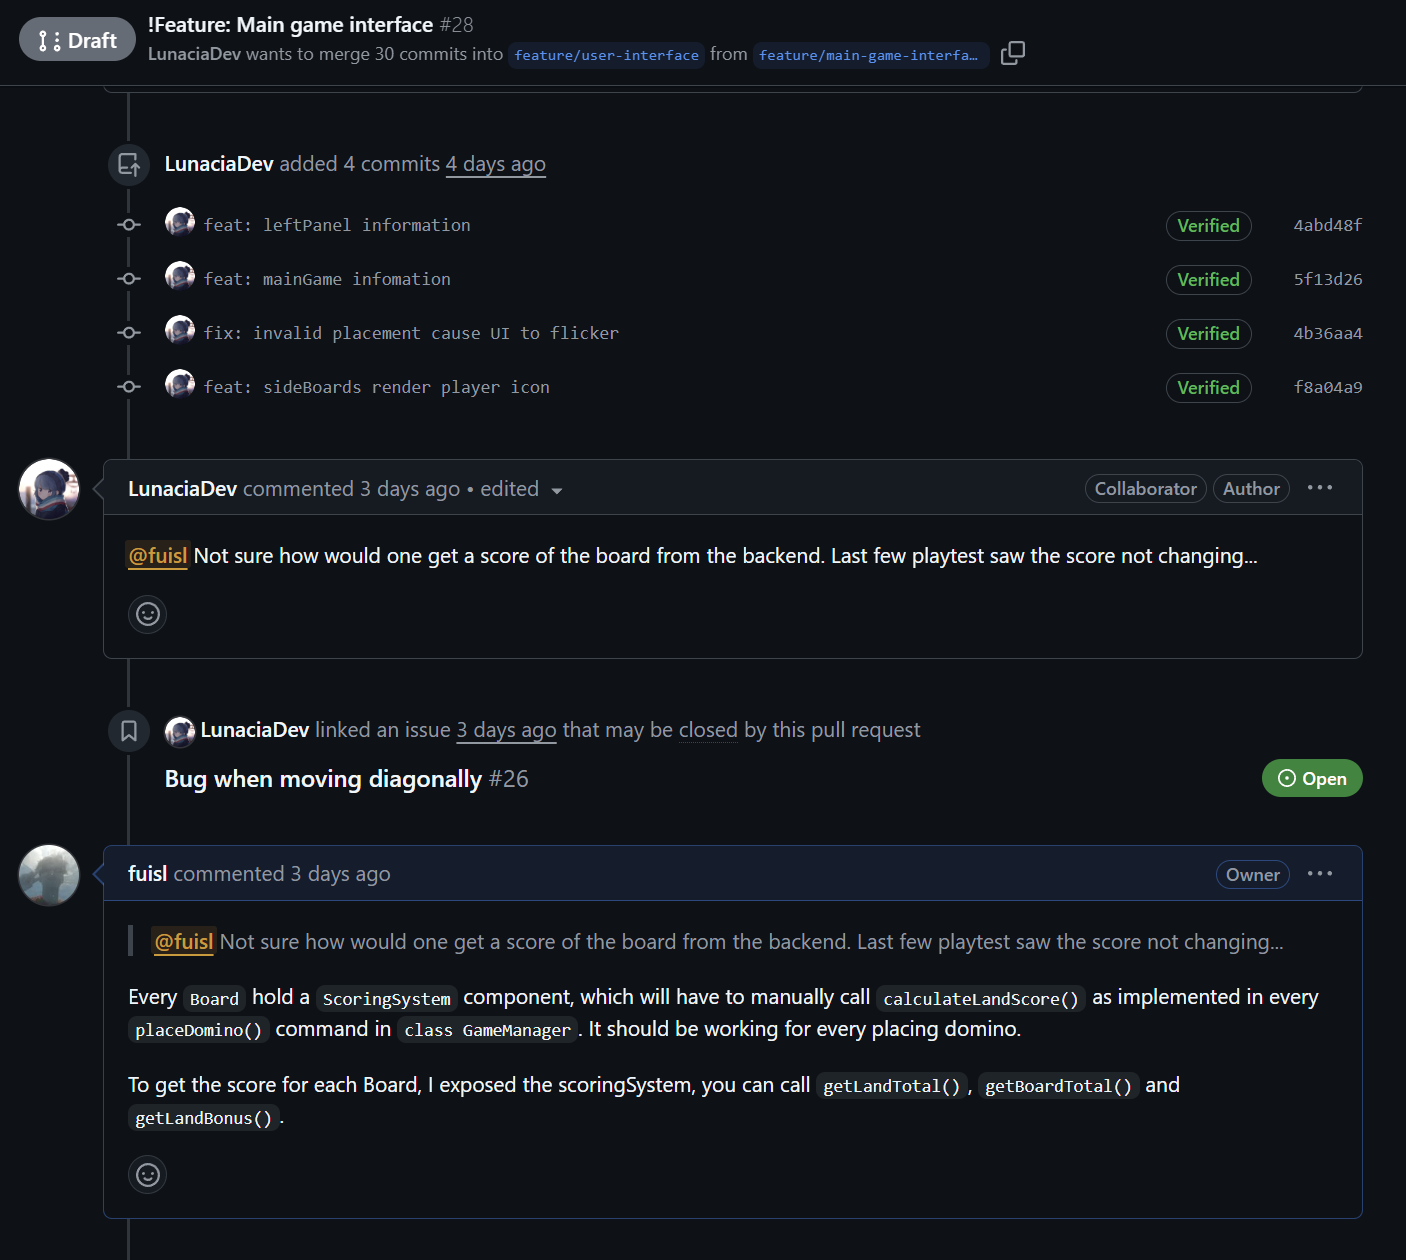
\includegraphics[width=0.48\textwidth]{assets/github-pr.png}}
    \caption{A conversation in one Pull Request.}\label{fig:github-pr}
\end{figure}

%======================================================
\section{Proposed Approaches}
\label{sec:proposed_approaches}

\subsection{Event-Driven Architecture}
% -- Explanation of the event-driven architecture, how is it involved in the game.

Kingdomino’s digital adaptation uses an event-driven architecture to manage
user interactions, game state transitions, and visual effects efficiently. This
approach decouples game logic, input handling, and rendering, improving
performance, modularity, and maintainability.

Although LibGDX does not explicitly provide an event-driven architecture, we
designed the game to integrate LibGDX's event handling system with our custom
event system, effectively implementing our own game engine. This hybrid
approach allows us to leverage LibGDX's rendering and input processing
capabilities while implementing our event-driven logic for custom background
tasks and UI interactions.

\subsection{Custom Game Engine}
\subsubsection{Event}
The \texttt{Event} class encapsulates actions that can be executed immediately
or after a delay. It supports different types of triggers:
\begin{itemize}
    \item \textbf{IMMEDIATE}: Executes the event as soon as it is created.
    \item \textbf{BEFORE}: Executes an action and then enforces a delay before completing.
    \item \textbf{AFTER}: Executes an action only after a specified delay.
    \item \textbf{CONDITION}: Executes when a certain condition is met.
    \item \textbf{EASE}: Implements smooth transitions for visual effects.
\end{itemize}
Each event has attributes such as blocking, blockable, complete, and delay, allowing for controlled execution within the game loop.

\subsubsection{EventManager}
The \texttt{EventManager} is the central hub for executing game events,
maintaining concurrent queues for:
\begin{itemize}
    \item \textbf{Base}: Core gameplay logic (turn transitions, score updates).
    \item \textbf{Input}: Player interactions (movement, rotation, placement).
    \item \textbf{Background}: Visual effects and animations.
    \item \textbf{Sound}: Audio effects (movement, tile placement, invalid moves).
    \item \textbf{Other}: Miscellaneous actions.
\end{itemize}
The event manager ensures concurrency safety using \texttt{ConcurrentLinkedQueue},
preventing race conditions when processing multiple asynchronous actions.\footnote{The event system may leak memory due to the creation of new events and their addition to the queue, but this is mitigated by garbage collection and the low trigger rate.}

\subsubsection{GameTimer}
The \texttt{GameTimer} class tracks real-time, total elapsed time, and
background animation timing. It synchronizes event execution by accumulating
delta time (dt) and updating event processing intervals accordingly. The timer
provides a consistent timing reference for executing delayed events and easing
functions.\footnote{The GameTimer accumulates time without resetting, which can
    eventually lead to an overflow if the game is left running for an extended
    period}

\subsubsection{Ease}
The \texttt{Ease} class facilitates smooth animations for background effects,
screen transitions, and UI enhancements. It supports different interpolation
methods:
\begin{itemize}
    \item \textbf{LERP (Linear Interpolation)}: Gradually changes a value over time.
    \item \textbf{ELASTIC}: Simulates spring-like motion for dynamic effects.
    \item \textbf{QUAD}: Creates a smooth acceleration effect.
\end{itemize}
This is particularly useful for animations such as screen shaking when an invalid move is made, or color transitions when switching player turns.

\subsection{Input Handling}
Kingdomino implements manual input event processing instead of relying on
LibGDX's built-in event loop. The input handling is divided into two main
components: \texttt{BoardInputController} and \texttt{BoardInputProcessor},
which handle input from controllers and keyboards, respectively. These
components translate user inputs into structured events that are processed by
the system.

\begin{figure}[htbp]
    \centerline{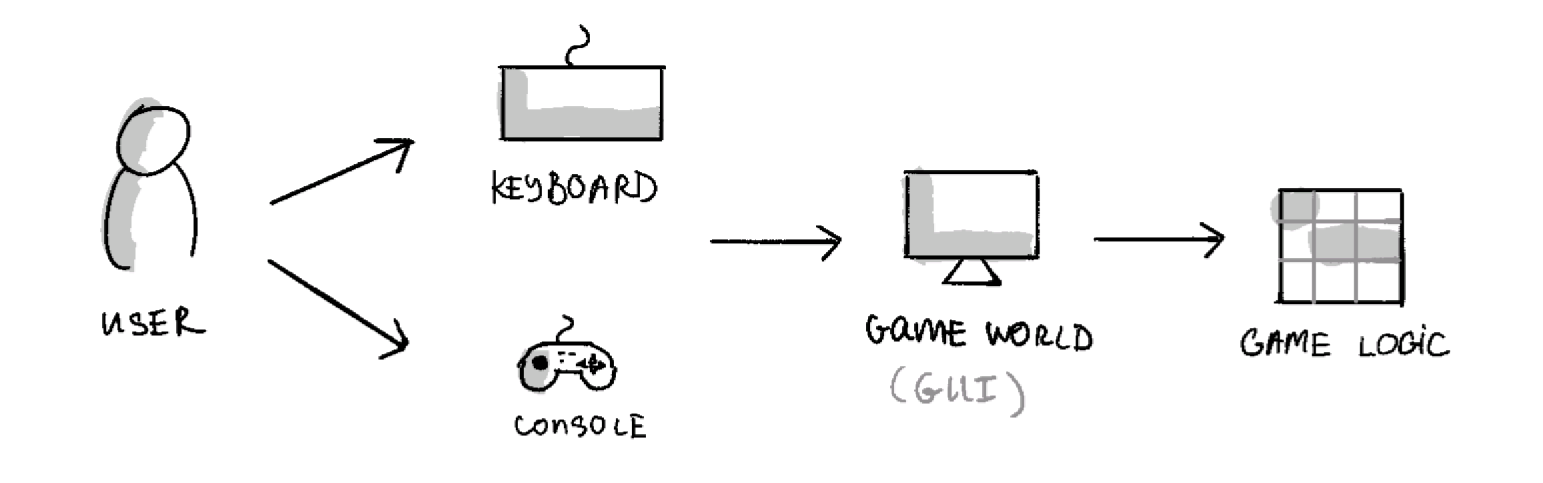
\includegraphics[width=0.5\textwidth]{assets/interaction.png}}
    \caption{Interfaces between user and game world.}\label{fig:interaction}
\end{figure}

\subsubsection{AbstractInputController}
The \texttt{AbstractInputController} class handles input from game controllers.
It captures axis movements and button presses, translating them into actions
such as moving, rotating, placing, or discarding a domino. The controller input
is processed with a dead zone to ignore small, unintended movements, ensuring
precise control.
\begin{lstlisting}[language=Java]
// filepath: /e:/projects/kingdomino/core/src/main/java/dev/kingdomino/game/AbstractInputController.java
package dev.kingdomino.game;

import com.badlogic.gdx.controllers.Controller;

public abstract class AbstractInputController implements ControllerListener {
    @Override
    public boolean buttonDown(...) { return handleStatus; }

    @Override
    public boolean buttonUp(...) { return handleStatus; }

    @Override
    public boolean axisMoved(...) { return handleStatus; }
}
\end{lstlisting}

\subsubsection{AbstractInputProcessor}
The \texttt{AbstractInputProcessor} class implements the
\texttt{InputProcessor} interface with all input events from keyboard. It is
being rejected by default. Specific input events can be handled by extending
this class and overriding the relevant methods.

\begin{lstlisting}[language=Java]
// filepath: /e:/projects/kingdomino/core/src/main/java/dev/kingdomino/game/AbstractInputProcessor.java
package dev.kingdomino.game;

import com.badlogic.gdx.InputProcessor;

public abstract class AbstractInputProcessor implements InputProcessor {
    @Override
    public boolean keyDown(int keycode) {return false;}

    @Override
    public boolean keyUp(int keycode) {return false;}
    // ...existing code...
}
\end{lstlisting}

\subsubsection{Input Handlers}
The \texttt{BoardInputHandler} and \texttt{DraftInputHandler} classes are
responsible for translating the inputs received from instance of
\texttt{AbstractInputController} and \texttt{AbstractInputProcessor} into
signals that the system can process. These handlers manage the state of the
game and ensure that inputs are processed correctly based on the current game
state.

\begin{lstlisting}[language=Java]
// filepath: /e:/projects/kingdomino/core/src/main/java/dev/kingdomino/game/BoardInputHandler.java
public class BoardInputHandler {
    // ...existing code...
    public boolean keyDown(Action action) {
        if (gameManager.getCurrentState() != GameManager.GameState.TURN_PLACING) {
            return false;
        }
        update(); // update states
        Event e = null;
        switch (action) {
                // ...existing code...
            case MOVE_RIGHT:
                // ...existing code...
            case ROTATE_CLOCKWISE:
                // ...existing code...
            case PLACE_DOMINO:
                // ...existing code...
            case DISCARD_DOMINO:
                // ...existing code...
            default:
                break;
        }
        if (e != null) {
            eventManager.addEvent(e.copy(), "input", false);
            updated = true;
        }
        return true; // returning true indicates the event was handled
    }
    // ...existing code...
}
\end{lstlisting}

To get the event from the input, each input has to translate the keycode into a
corresponding action using the /texttt{translateKeycodeToAction} method, which
maps specific key presses to game actions such as moving, placing, or
discarding a domino.

Simmilarly, \texttt{DraftInputHandler} class handles translated input events
for selecting next dominoes.

\begin{lstlisting}[language=Java]
// filepath: /e:/projects/kingdomino/core/src/main/java/dev/kingdomino/game/DraftInputHandler.java
public boolean keyDown(Action action) {
    // ...existing code...
    switch (action) {
        case MOVE_UP:
            // ...existing code...
        case MOVE_DOWN:
            // ...existing code...
        case SELECT_DOMINO:
            // ...existing code...
        default:
            break;
    }
    //...existing code...
}
\end{lstlisting}

\subsubsection{Key Features of Input Handling}
The input handling system in Kingdomino features deferred execution, where
actions are queued and processed asynchronously, state-based processing that
ensures input is handled only in relevant game states, and feedback integration
that triggers audio and visual feedback for invalid actions.

\subsubsection{Input Handling}
The input handling system in Kingdomino features deferred execution, where actions are queued and processed asynchronously, state-based processing that ensures input is handled only in relevant game states, and feedback integration that triggers audio and visual feedback for invalid actions.
\begin{algorithm}[htbp]
    \caption{Handling Movement Events}
    \KwIn{Player input (WASD keys or joystick)}
    \KwOut{Updated domino position}
    \Begin{
        Capture player input\;
        \If{Input is valid}{
            Create a move event with delay for smooth input\;
            \texttt{moveEvent} $\leftarrow$ \texttt{new Event(TriggerType.BEFORE, true, true, 0.15, () -> currentDomino.moveDomino(Direction.UP), null, null, null)}\;
            Add event to event manager queue\;
            \texttt{eventManager.addEvent(moveEvent, "input", false)}\;
            Play sound effect for invalid move\;
            \texttt{audioManager.playSound(AudioManager.SoundType.CANCEL)}\;
            Trigger screen shake effect\;
            \texttt{BackgroundManager.screenShake()}\;
        }
    }
\end{algorithm}

\subsection{User Interface}

\subsubsection{User Interface Layout Design}

We chose to design the user interface based on tables, where each component or
table is placed within a cell as demonstrated in \ref{fig:ui-proto}.

\begin{figure}[htbp]
    \centerline{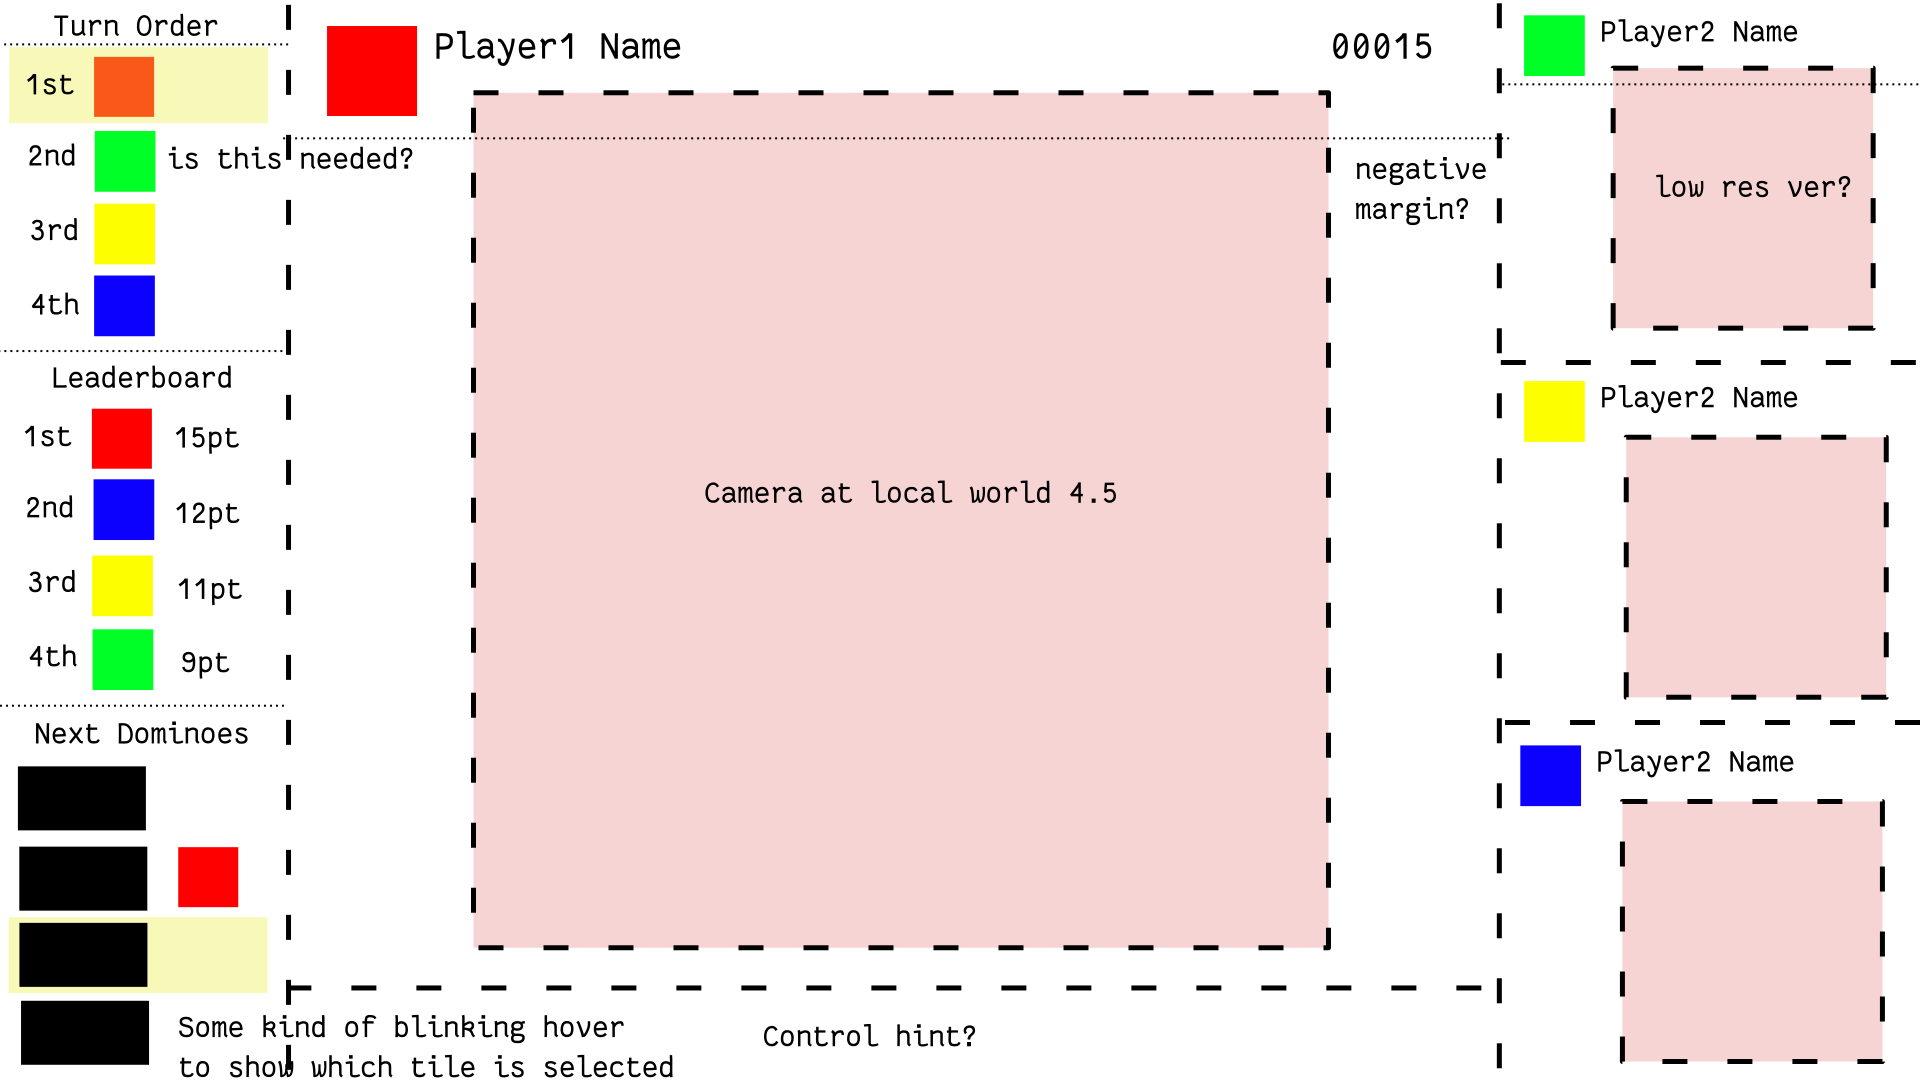
\includegraphics[width=0.48\textwidth]{assets/ui-prototype.png}}
    \caption{First UI design prototype.}\label{fig:ui-proto}
\end{figure}

We mimic how the game state of Kingdomino is distributed in real life by having
the current player's game board being placed prominently in the center of the
screen, whilst other informations that the player can find are placed to the
side. We also decided to show how many points each player is currently scoring
with their board as well, because it could enable more strategic choice if
players know exactly how their board is doing compared to other, instead of
focusing on picking the tile that would yield the most point for their board.

%======================================================
\section{Implementation Details}
\label{sec:implementation_details}
% 6. IMPLEMENTATION DETAILS
% -- Application structure, GUI details, UML/Class Diagram, used libraries, important code snippets.

\subsection{Game States}

In the implementation of Kingdomino, the game progresses through a series of
well-defined states. Each state represents a distinct phase of the game,
ensuring a structured flow from the beginning to the end. The primary game
states include:

\begin{itemize}
    \item \textbf{Init}: The initial state where the game components are set up and initialized.
    \item \textbf{Setup}: This state involves preparing the game board, shuffling tiles, and setting up players for the game.
    \item \textbf{Turn Start}: Marks the beginning of a player's turn, where the current player and available tiles are determined.
    \item \textbf{Turn Placing}: The state where the player places their selected tile on the board according to the game rules.
    \item \textbf{Turn Choosing}: The state where the player selects a tile for the next round.
    \item \textbf{Turn End}: Concludes the current player's turn and transitions to the next player.
    \item \textbf{Game Over}: The final state when the game ends, and no more moves can be made.
    \item \textbf{Results}: Displays the final scores and determines the winner based on the game rules.
\end{itemize}

Each state transitions to the next based on player actions and game logic. The
following diagram illustrates the state transitions:

\begin{figure}[htbp]
    \centerline{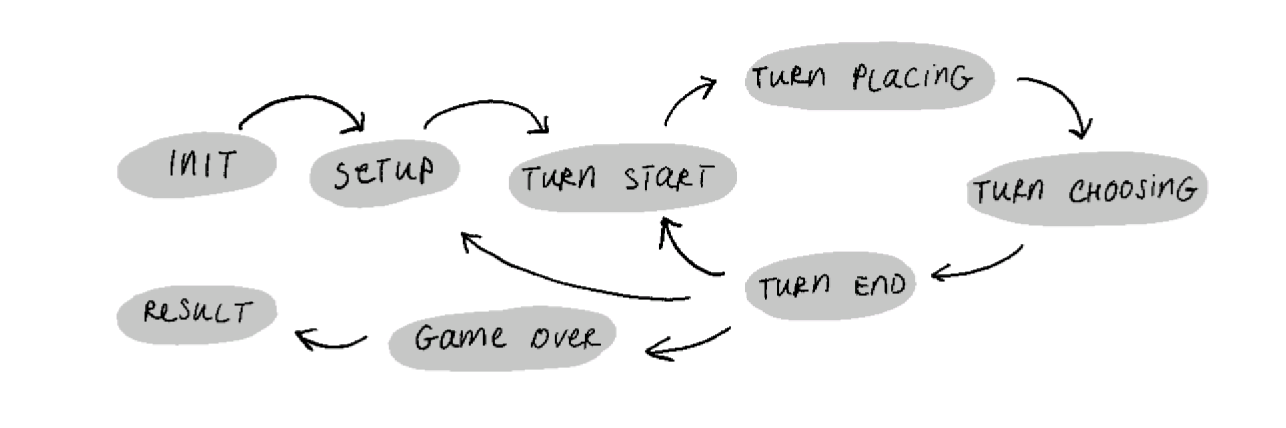
\includegraphics[width=0.55\textwidth]{assets/states.png}}
    \caption{Game State Transitions.}\label{fig:game_states}
\end{figure}

\subsection{Game Units and High-Level Architecture}
% -- High-level architecture. Possibly a diagram.

Tile is the essential, smallest accessible unit for this game. Tile holds 2
most important attributes: TerrainType and Number of Crowns.

\begin{figure}[htbp]
    \centerline{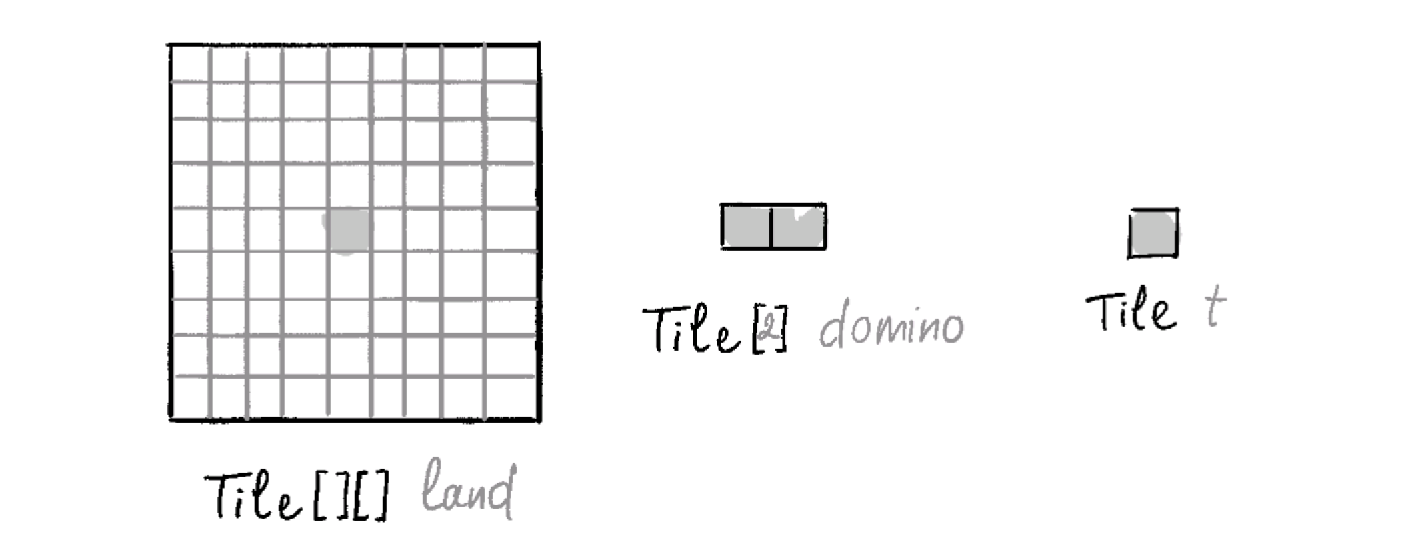
\includegraphics[width=0.48\textwidth]{assets/unit.png}}
    \caption{Units of Tile.}\label{fig:unit}
\end{figure}

Board is 2-dimensional array of type Tile. Though Board has more attributes and
methods which supports interactions between GameManager and Board, Tile[][] is
where Tiles being store and perform logic on.

On the other hand, Domino is an interface between human player and Board. It
holds informations about location, validator, etc., which related to action
that can be performed on Board (like moving, rotating or placing Domino). The
actual Domino will not be placed in Board, only the two Tiles that composes
Domino would be added. Domino will then be discarded.

\subsection{Tile Placement and Board Validation}

\subsubsection{Domino and DominoController}

The \texttt{Domino} class represents a domino in the game, consisting of two
tiles and a controller. It provides methods to rotate, move, and set the
position of the domino. The \texttt{DominoController} class handles the
rotation and placement of dominos, maintaining the state of the tiles and their
positions.

\begin{figure}[htbp]
    \centerline{
        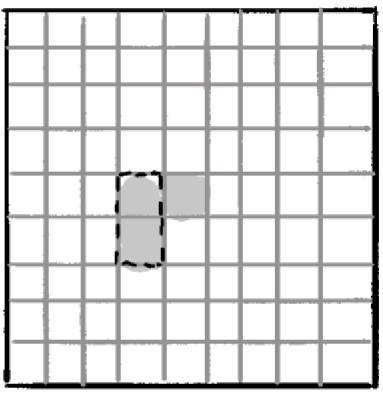
\includegraphics[width=0.18\textwidth]{assets/placing-1.png}
        \hspace{0.01\textwidth}
        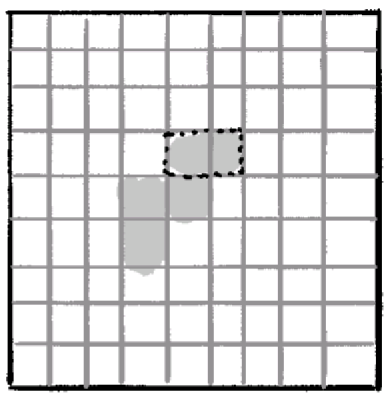
\includegraphics[width=0.18\textwidth]{assets/placing-2.png}
    }
    \caption{Placing Domino.}\label{fig:placing}
\end{figure}

\begin{lstlisting}[language=Java]
// filepath: /e:/projects/kingdomino/core/src/main/java/dev/kingdomino/game/Domino.java
public class Domino {
    // ...existing code...
    public void rotateDomino(boolean clockwise, boolean shouldOffset) {
        dominoController.rotateDomino(clockwise, shouldOffset);
    }
    // ...existing code...
}
\end{lstlisting}

\begin{lstlisting}[language=Java]
// filepath: /e:/projects/kingdomino/core/src/main/java/dev/kingdomino/game/DominoController.java
public class DominoController {
    // ...existing code...
    public void rotateDomino(boolean clockwise, boolean shouldOffset) {
        lastRotationIndex = rotationIndex;
        rotationIndex = (rotationIndex + (clockwise ? 1 : 3)) % 4;

        // rotate the 2nd Tile with 1st Tile as center
        tileRotator.rotate(posTileA, posTileB, rotationIndex, shouldOffset);

        lastAction = 1;
    }
    // ...existing code...
}
\end{lstlisting}

\subsubsection{TileRotator}

The \texttt{TileRotator} class is responsible for rotating tiles around a
center position. It uses a predefined set of directions to determine the new
position of the tile after rotation.

\begin{figure}[htbp]
    \centerline{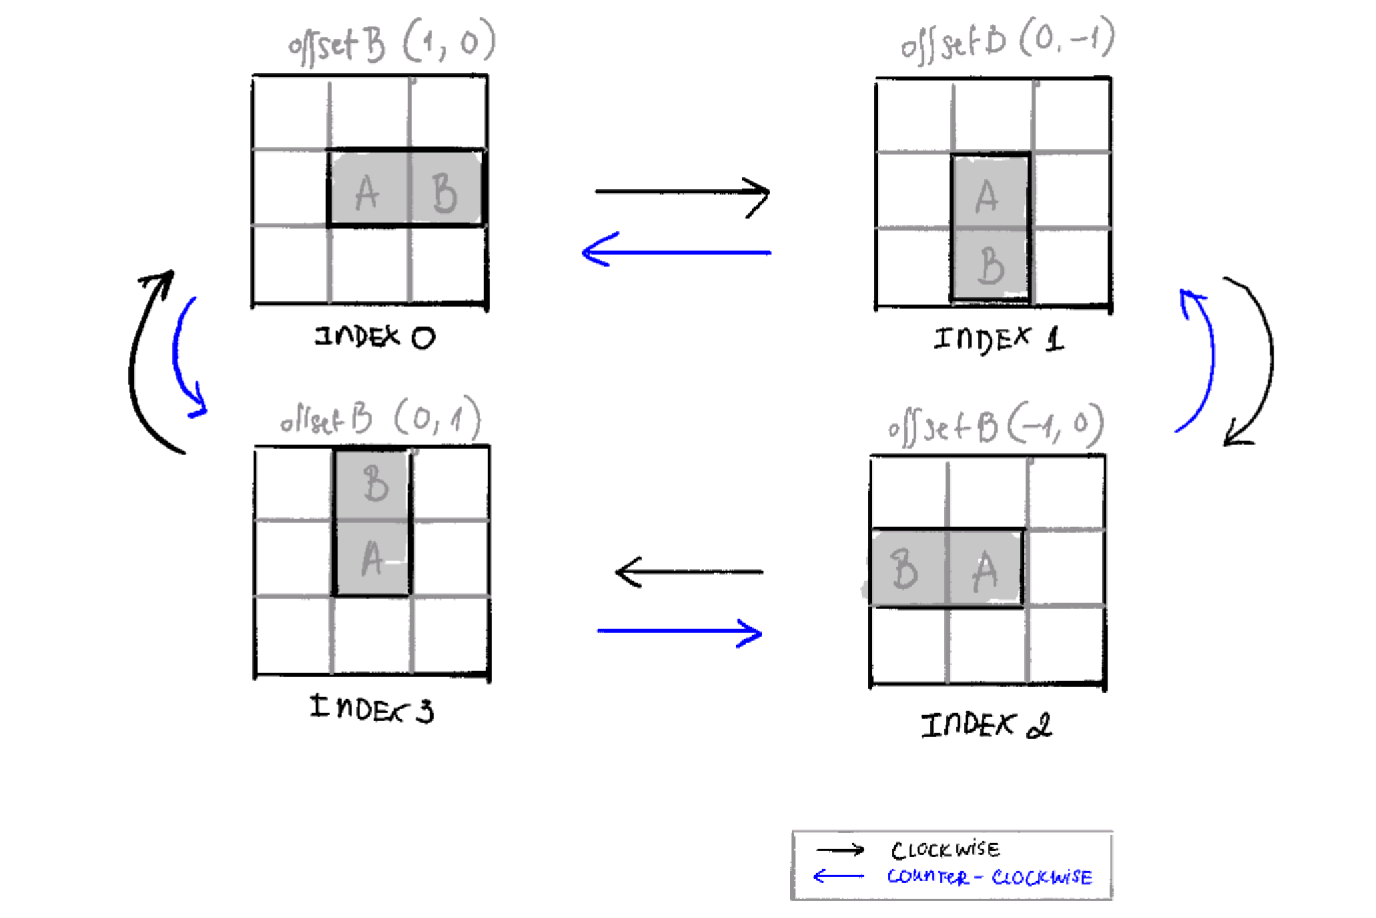
\includegraphics[width=0.55\textwidth]{assets/rotate.png}}
    \caption{Rotate Domino by moving TileB relative to TileA.}\label{fig:rotate}
\end{figure}

The rotation logic for the domino can be described as follows:

\[
    \text{If rotating clockwise:} \quad\boxed{\text{index} = (\text{index} + 1) \mod 4}
\]
\[
    \text{If rotating counter-clockwise:} \quad\boxed{\text{index} = (\text{index} + 3) \mod 4}
\]

\begin{lstlisting}[language=Java]
// filepath: /e:/projects/kingdomino/core/src/main/java/dev/kingdomino/game/TileRotator.java
public class TileRotator {
    // ...existing code...
    public void rotate(Position center, Position tilePos, int rotationIndex, boolean shouldOffset) {
        Position newPos = center.add(directions[rotationIndex]);
        tilePos.set(newPos);
    }
    // ...existing code...
}
\end{lstlisting}

\subsubsection{Tile Placement Validation}

The \texttt{TileValidator} class is responsible for validating the placement of
tiles on the game board. It ensures that tiles are placed within bounds and are
free from occupation. The following code snippet shows the implementation of
the \texttt{TileValidator} class:

\begin{lstlisting}[language=Java]
// filepath: /e:/projects/kingdomino/core/src/main/java/dev/kingdomino/game/TileValidator.java
public class TileValidator {
    // ...existing code...
    public boolean isTilePlaceable(Tile tile, int x, int y) {
        return isTileFree(x, y) && isTileWithinBound(x, y);
    }
    // ...existing code...
    public boolean isTileWithinBound(int x, int y) {
        if (x < minX || x > maxX) {
            if (abs(x - minX) + 1 > size || abs(x - maxX) + 1 > size) {
                return false;
            }
        }
        if (y < minY || y > maxY) {
            if (abs(y - minY) + 1 > size || abs(y - maxY) + 1 > size) {
                return false;
            }
        }
        return true;
    }
    // ...existing code...
    public boolean isTileFree(int x, int y) {
        if (isTileWithinLand(x, y)) {
            return land[y][x] == null;
        }
        return false;
    }
    // ...existing code...
}
\end{lstlisting}

\subsection{Scoring Mechanism}
% -- Explain the flood-fill algorithm and its application in Kingdomino.

The flood-fill algorithm is a computer graphics algorithm used to determine the
area connected to a given node in a multi-dimensional array. It is commonly
used in tools like paint bucket in graphics editors to fill bounded areas with
color.

In the context of Kingdomino, the flood-fill algorithm is utilized to calculate
the score by identifying and evaluating connected groups of the same terrain
type. The algorithm traverses the game board, starting from a given tile, and
recursively explores all adjacent tiles of the same terrain type. This allows
the game to efficiently compute the size of each connected terrain group and
apply the scoring rules based on the number of crowns within these groups.

Below is a pseudocode representation of the recursive 4-way flood-fill
algorithm:

\begin{algorithm}[htbp]
    \caption{Flood-fill Algorithm}
    \KwIn{Tile}
    \KwOut{Flood-filled region}
    \If{Tile is not inside Region}{
        \Return\;
    }
    Set the node\;
    Perform Flood-fill one step to the south of Tile\;
    Perform Flood-fill one step to the north of Tile\;
    Perform Flood-fill one step to the west of Tile\;
    Perform Flood-fill one step to the east of Tile\;
    \Return\;
\end{algorithm}

This algorithm is in its original form. For Kingdomino with multiplicative
scoring system, we need to modify the algorithm to calculate both the spanned
region (area) and also count the number of crowns within the connected group.
See Listing~\ref{lst:floodfill} for the implementation details.

To better illustrate the concept of flood-fill, consider the following example
with a 9$\times$9 grid:

\begin{figure}[htbp]
    \centerline{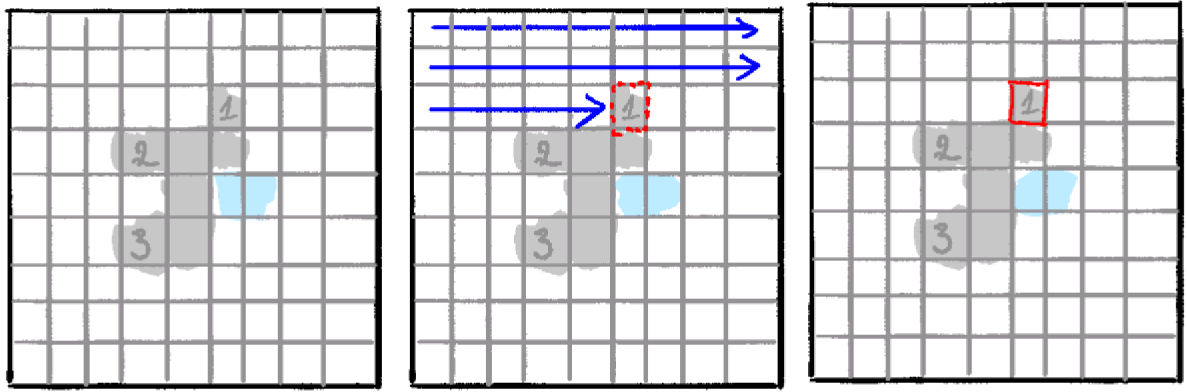
\includegraphics[width=0.48\textwidth]{assets/floodfill-start.png}}
    \centerline{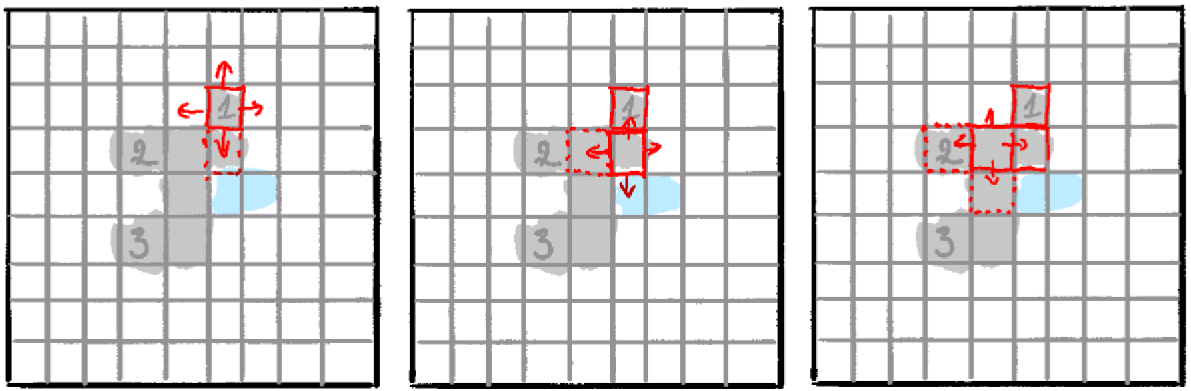
\includegraphics[width=0.48\textwidth]{assets/floodfill-detected.png}}
    \centerline{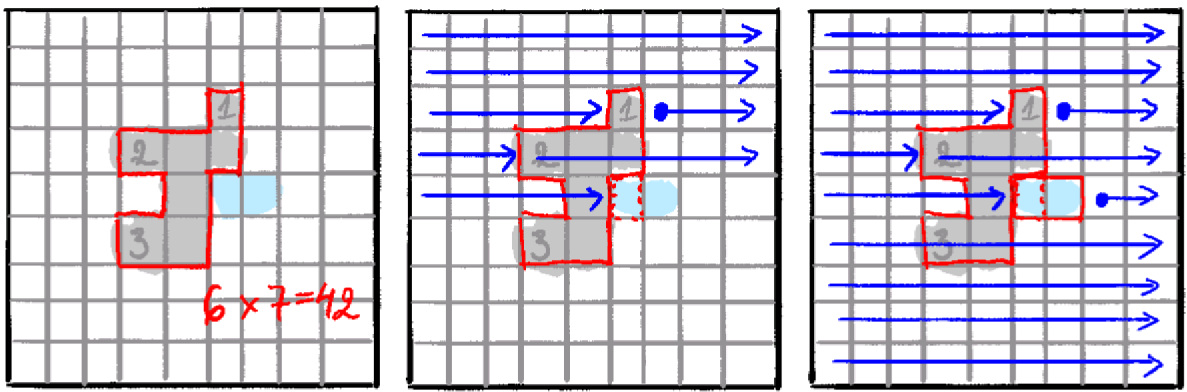
\includegraphics[width=0.48\textwidth]{assets/floodfill-continue.png}}
    % \caption{}\label{fig:floodfill-start}
\end{figure}

In this example, the algorithm starts at the selected tile (highlighted in
red). It then recursively explores all adjacent tiles of the same terrain type,
marking them as visited and counting the number of crowns within the connected
group. The process continues until all connected tiles of the same terrain type
have been evaluated, resulting in the final score for that terrain group.

Below is the actual implementation of the flood-fill algorithm in Kingdomino:

\begin{lstlisting}[language=Java, caption={Flood-Fill Algorithm}, label={lst:floodfill}]
    private int floodFill(int x, int y, TerrainType terrain, boolean[][] visited) {
        if (x < 0 || x >= land.length || y < 0 || y >= land.length) {
            return 0;
        }
    
        if (land[y][x] == null || visited[y][x] || land[y][x].getTerrain() != terrain) {
            return 0;
        }
        
    
        totalCrown += land[y][x].getCrown();
        visited[y][x] = true;
    
        return 1 +
                floodFill(x + 1, y, terrain, visited) +
                floodFill(x - 1, y, terrain, visited) +
                floodFill(x, y + 1, terrain, visited) +
                floodFill(x, y - 1, terrain, visited);
        }
    \end{lstlisting}

\subsection{UML/Class Diagram}
% -- Provide an overview of classes, relationships. 
%    Reference the figure in text.

\subsection{Used Libraries and Environment}
% -- Mention languages, frameworks, libraries, operating systems, version details, etc.

%======================================================
% -- mainly UI

\section{Graphical Enhancement and Visual Effects}
% 8. GRAPHICAL ENHANCEMENT AND VISUAL EFFECTS
\label{sec:graphical_enhancement}
% -- Describe the interface design, layout, main widgets.

\subsection{Visual and Effects}
Kingdomino's digital adaptation incorporates various visual and audio effects
to enhance the user experience, making the game feel more responsive and
engaging. Inspired by the talk ``Juice it or lose it'' by Martin Jonasson \&
Petri Purho, we aimed to create a game that feels alive and responds to player
actions with minimal input.

\subsubsection{Background Effects}
The \texttt{BackgroundManager} class manages dynamic background effects using
shader-based rendering. Key features include:
\begin{itemize}
    \item \textbf{Color Transitions}: Smooth transitions between different background colors to indicate changes in game states or player turns.
    \item \textbf{Spinning Effects}: Controlled spinning of the background to add a sense of motion and excitement during gameplay.
    \item \textbf{Screen Shake}: A subtle screen shake effect to provide feedback for significant events, such as invalid moves or special actions.
\end{itemize}

\subsubsection{Audio Effects}
The \texttt{AudioManager} class handles the game's audio effects, providing
immediate feedback for player actions. Key features include:
\begin{itemize}
    \item \textbf{Background Music}: Continuous background music that sets the tone for the game.
          % -- SFX is used in order to provide immediate feedback, as often time it is not obvious that something have happened when the user interact with the game.
    \item \textbf{Sound Effects}: Various sound effects for actions such as tile placement, selection, rotation, and scoring in order to provide immediate feedback for each action the player take.
\end{itemize}

\subsubsection{Shader-Based Rendering}
Kingdomino leverages shader-based rendering using OpenGL Shader language to
enhance visual effects and provide a more immersive experience. Two primary
shaders are used: the CRT shader and the background shader. The shader codes
are an adaptation of existing shaders of Balatro\cite{wiki:balatro} which
adapted from Löve2D written in Lua to LibGDX Framework using with Java.

\paragraph{CRT Shader}
The CRT shader simulates the appearance of an old CRT monitor, adding effects
such as distortion, scanlines, noise, and bloom. It consists of a vertex shader
and a fragment shader.

\begin{itemize}
    \item \textbf{Vertex Shader (crt.vert)}: Applies transformations to simulate a parallax effect based on screen scale.
    \item \textbf{Fragment Shader (crt.frag)}: Implements various visual effects, including barrel distortion, edge feathering, glitch offsets, chromatic aberration, scanlines, and noise overlay.
\end{itemize}

\paragraph{Background Shader}
The background shader creates dynamic and visually appealing backgrounds with
effects like spinning and color transitions.

\begin{itemize}
    \item \textbf{Vertex Shader (background.vert)}: Passes texture coordinates to the fragment shader.
    \item \textbf{Fragment Shader (background.frag)}: Applies pixelation, swirl, and paint effects based on time and spin parameters, along with color blending for a vibrant background.
\end{itemize}

These visual and audio enhancements contribute to a more engaging and immersive
gaming experience, making Kingdomino not just a digital adaptation but a lively
and responsive game that captivates players.

\subsection{Game Textures}

Aside from the image of the King which was taken by Adam Carmichael
\cite{github:carmichael-repo} and the font Pixelify Sans
\cite{github:pixelify-sans}, all of the game's texture are hand-drawn. The tile
are created from a 48x48 pixel square of the color representative of its
terrain type, before applying Perlin Noise \cite{wiki:perlin-noise} so as to
reduce the monotonousness of the texture. We delibrately choose low texture
size as large, detailed texture would become inelligible by the CRT Shader.

\begin{figure}[htbp]
    \centerline{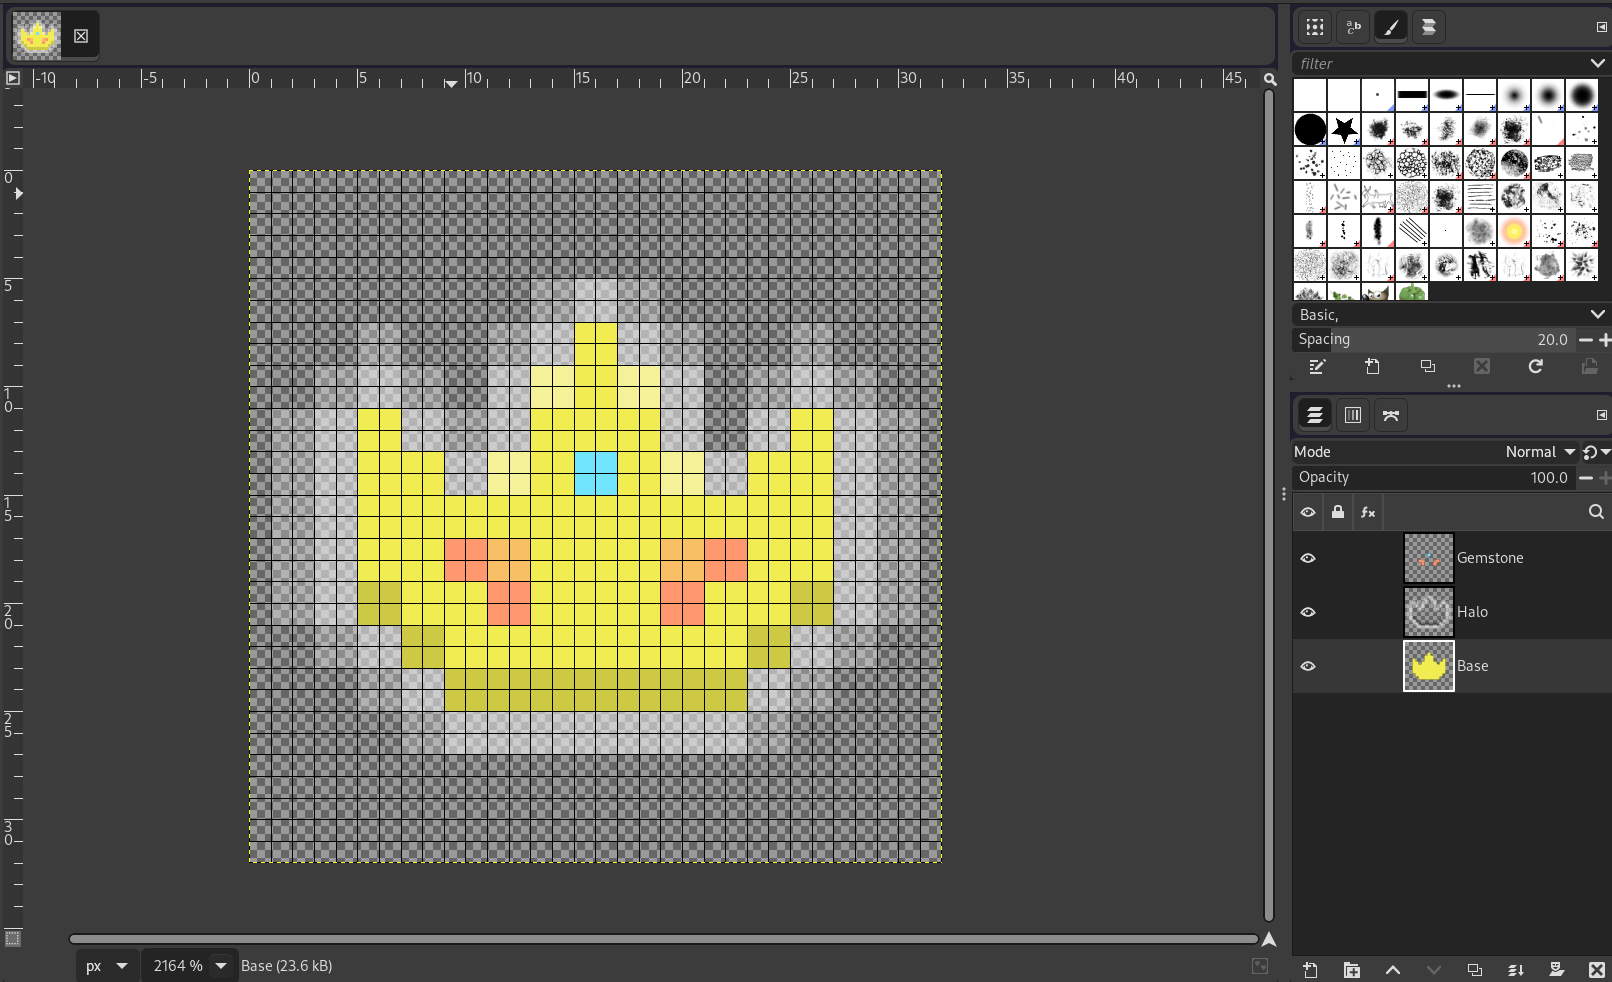
\includegraphics[width=0.48\textwidth]{assets/crown-design-file.png}}
    \caption{Original design file of the Crown.}\label{fig:crown-design}
\end{figure}

%======================================================
\section{Experimental Results}
\label{sec:experimental_results}
% 7. EXPERIMENTAL RESULTS, STATISTICAL TESTS, RUNNING SCENARIOS
% -- Provide tables, charts, and discussion of the experiments you ran.

\subsection{Performance Analysis}
% -- Discuss the performance of the game, any bottlenecks, optimizations.
framerate, input lag event-driven vs. sync update

\subsection{Correctness and Scalability}
% -- Describe your environment, parameter choices, etc.

\subsection{UI/Gameplay Smoothness}
% -- Insert tables and charts with relevant data and evaluations.

% \begin{table}[htbp]
% \caption{Example of Results Table}
% \begin{center}
% \begin{tabular}{|c|c|c|}
% \hline
% \textbf{Parameter} & \textbf{Value / Range} & \textbf{Observation}\\
% \hline
% Population Size & 50--200 & Performance improved \\
% Mutation Rate   & 5\%     & Minimal difference \\
% \hline
% \end{tabular}
% \label{tab:results}
% \end{center}
% \end{table}

%======================================================
\section{Conclusions and Future Work}
\label{sec:conclusions}
% 8. CONCLUSIONS AND FUTURE WORK
% -- Discuss overall findings, reflect on teamwork, 
%    lessons learned, and possible future improvements.

Lorem ipsum dolor sit amet, consectetur adipiscing elit.

\subsection{What We Learned}
% -- Key lessons from implementing or analyzing the game.

\subsection{Future Development}
% -- Potential expansions, new game modes, new algorithms, etc.

%======================================================
\appendices%
\section{Gameplay Mechanic}\label{app:gameplay}
% -- Provide additional content that supports the main text.

%======================================================
% -- Follow the IEEE reference style
% -- Cite references in text, e.g., [1], [2], etc.

\bibliographystyle{IEEEtran}
\bibliography{bibliography}

\end{document}
